\documentclass[a4paper, comsoc]{IEEEtran}
\usepackage[T1]{fontenc}
\usepackage{graphicx}
\graphicspath{{figs/}}

\IEEEoverridecommandlockouts

\usepackage{amsmath,amssymb,amsfonts}
\usepackage{algorithmic}
\usepackage{textcomp}
\usepackage{xcolor}
\usepackage{lipsum}

\usepackage{hyperref}
\hypersetup{
    colorlinks=true,
    linkcolor=blue,
    filecolor=magenta,      
    urlcolor=teal,
    pdftitle={Iscc2023 Paper}
}
\usepackage{xurl}


\usepackage[style=ieee,doi=false,url=true]{biblatex}
\AtEveryBibitem{%
  \clearfield{note}%
}
\addbibresource{tebaka2023.bib}

\begin{document}    % 7 Pagine, Double Column

\title{TEBAKA: Territorial Basic Knowledge Acquisition. An Agritech Project for the Italy}
%\thanks{Tebaka thanks}
\author{\IEEEauthorblockN{Lorenzo Epifani, Antonio Caruso}\\
\IEEEauthorblockA{\textit{Dept. of Mathematics and Physics "Ennio de Giorgi", University of Salento, Lecce, Italy}}}

\maketitle

\begin{abstract}
Tebaka, proposal, impact, some work.
\end{abstract}

\begin{IEEEkeywords}
digital agriculture, precision agriculture, satellite images, deep learning, machine learning,
sensor networks and iot
\end{IEEEkeywords}


\section{Introduction}
% general intro to agritech and relevance for computer science.

The enabling technologies of distributed sensor networks, internet of things, remote sensing with multi-spectral cameras on satellites, drones and aerial platforms, together with smart decision support systems are key contributors for the emerging field of \emph{Digital Agriculture} (DA) or \emph{Agriculture 4.0} \cite{de2018agriculture}. 
This is an \emph{umbrella term} used to designate the transformation of farming that includes digitalization and automation of farming tasks. This area of research, encompass a new vision of the farming industry as a cyber-physical farm, and includes all technological areas such as: big-data platforms, machine learning and data-driven models to relate the observations of the phenological stages of plants with field yield and crop quality. 

The high-level goal is to support agronomist with \emph{Precision Agriculture} management practices, to better solve the challenges and demand of an increasing world-population, rising production costs (like energy), labor shortages, climate and environmental changes (like water resource scarcity). It leverage extensive knowledge acquisition using remote sensing technologies, and on-the-field deployment of sensors and iot networks, to improve knowledge acquisition and situated situation awareness, to maximize resource usage and crop yield while minimizing associated costs.

In the United States, the use of yield-maps and soil maps are adopted only by 5 to 25 percent of total U.S. farms; on the other hand, automated guidance, has increased sharply, with the advance in deep-learning applied to computer vision, and it is applied to over 50 percent of the cultivated areas. A good survey of the trend in the technology evolution of a \emph{Smart Farm} in U.S. is in \cite{mcfadden2023precision}. USDA (The U.S. Department of Agriculture) is investing up to $2.8$ billion in $70$ selected projects under the first Partnerships for Climate-Smart Commodities funding pool, as a part of the Inflaction Reduction Act.


\begin{figure}
    \centering
    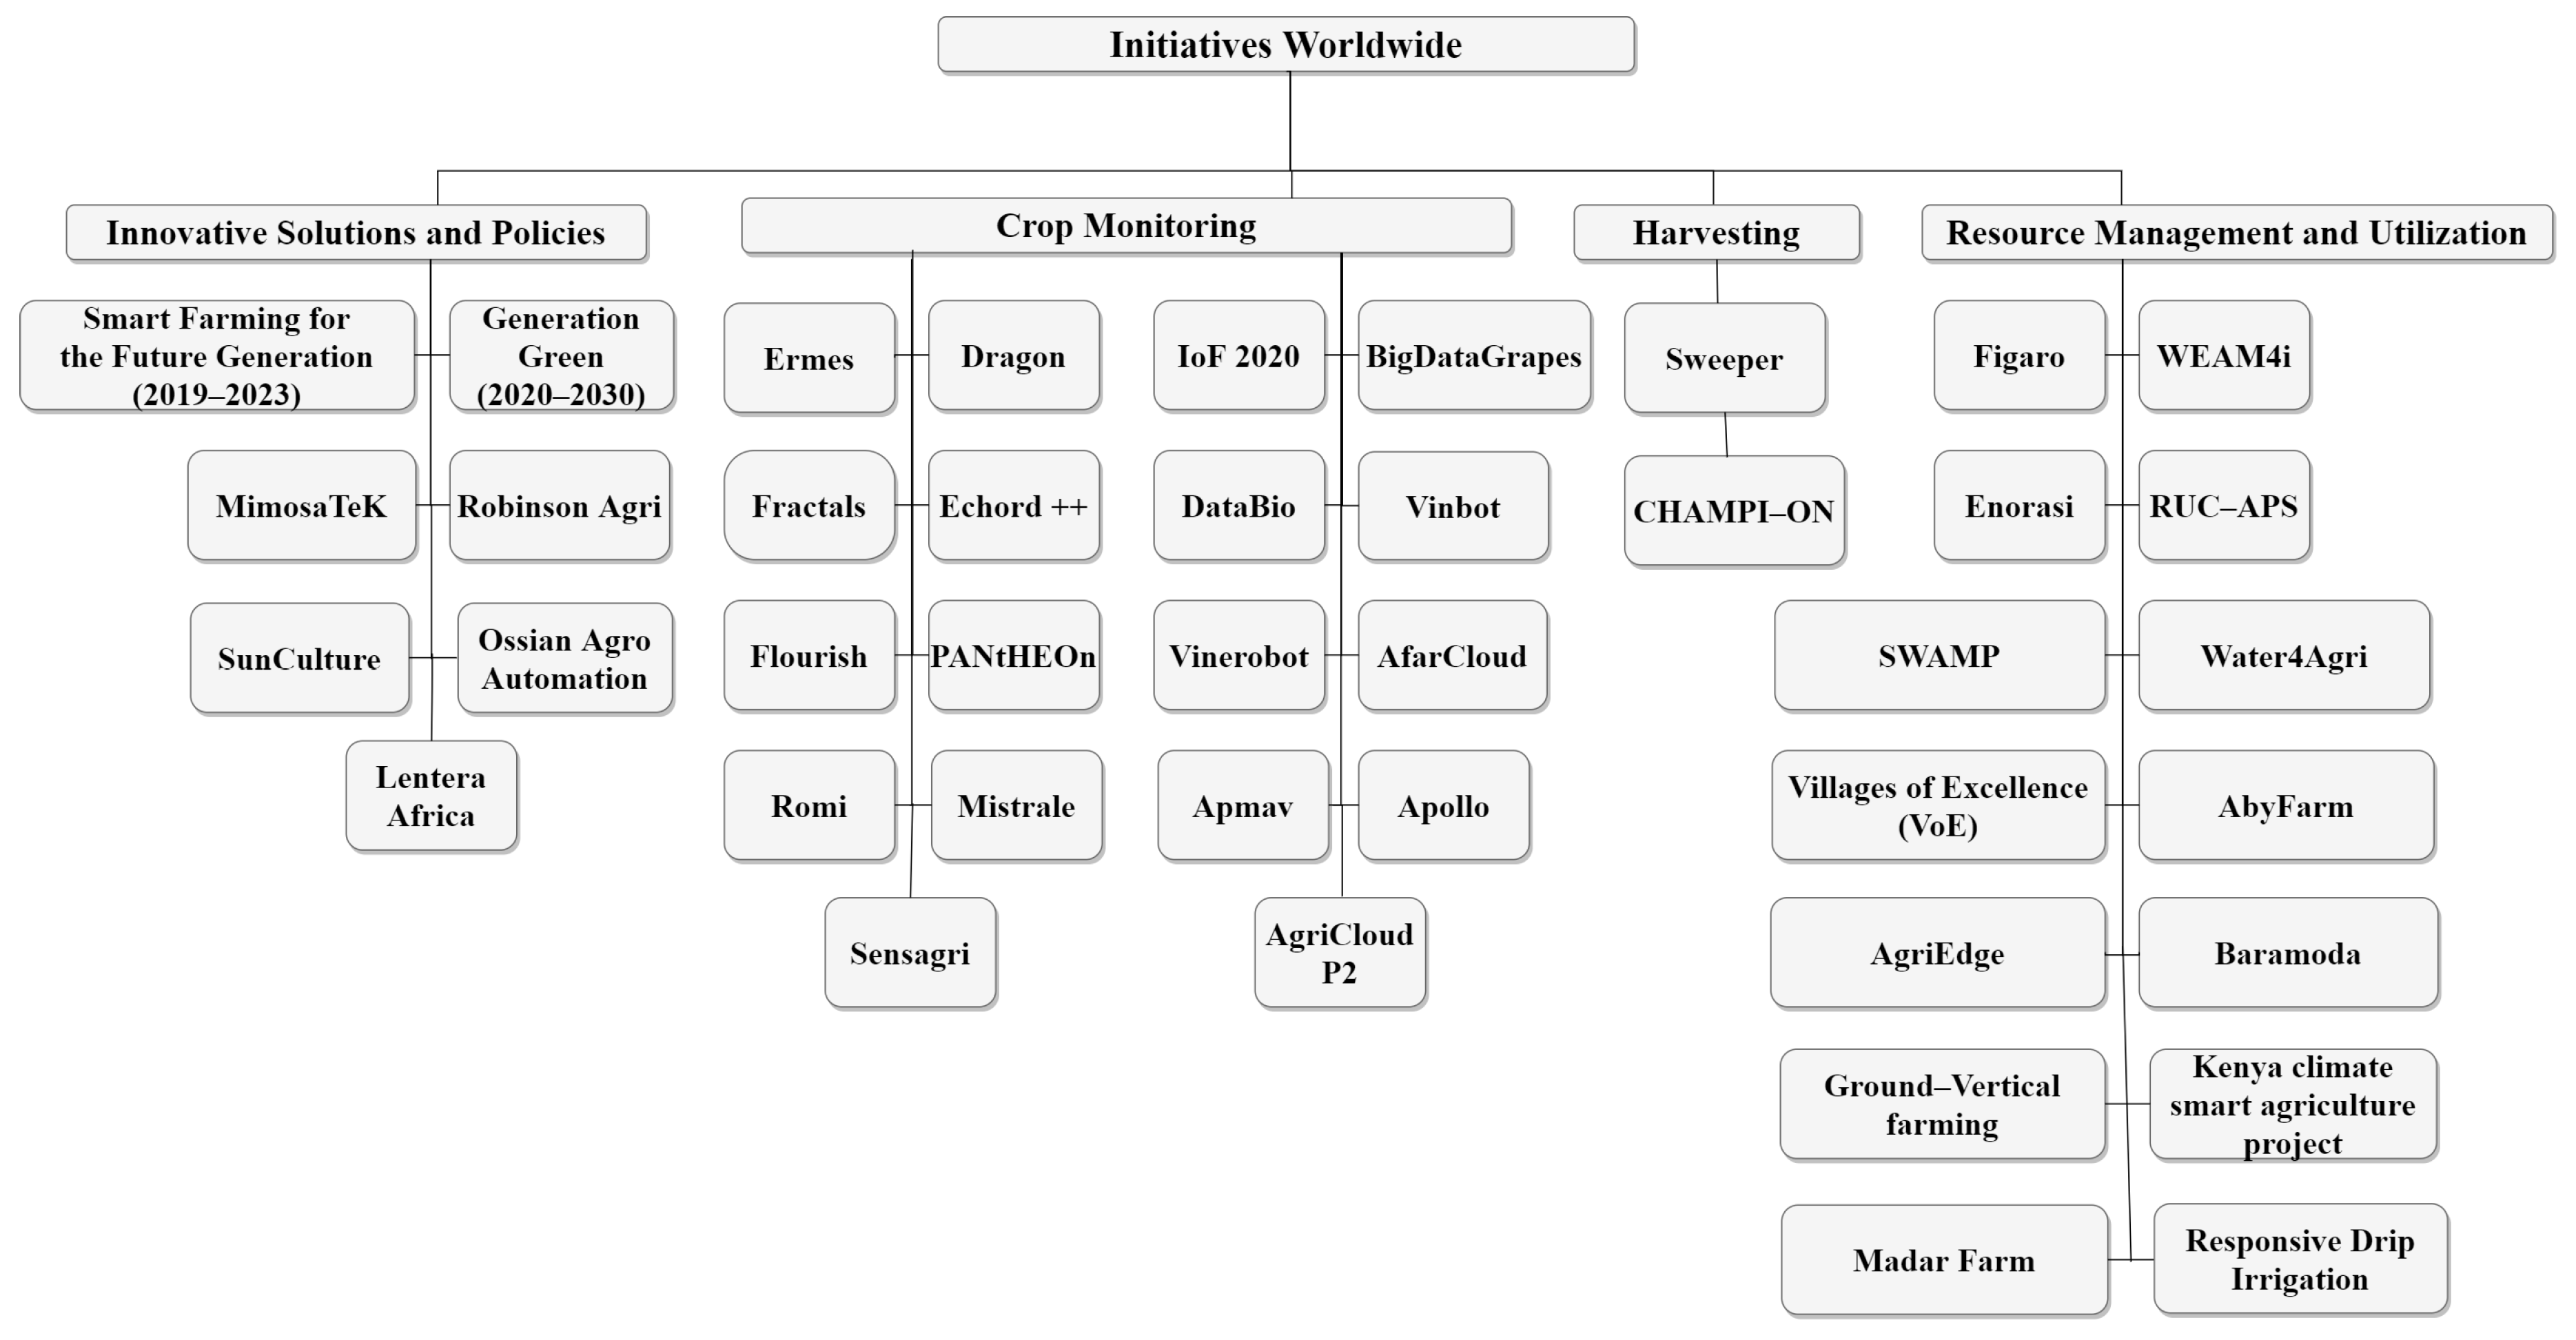
\includegraphics[width=\columnwidth]{agriengineering-04-00029-g005}
    \caption{A classification of active European Union funded project in the area of Digital Agriculture (from \cite{agriengineering4020029})}
    \label{fig:euprojects}
\end{figure}

In Europe, the European Community has funded many project that integrate ICT technologies and Digital Argriculture, we see in Figure \ref{fig:euprojects} from \cite{agriengineering4020029} a collection of active research project and startups, classified in different areas, such as:  \emph{Crop Monitoring}  (the largest one), \emph{Harvesting}, optimization of \emph{Resource Managements} and \emph{Innovative Policies and Solutions} with more than $41$ iniziatives. In Table \ref{fig:table-worldwide} another list of worldwide projects that are actually funded, with a major role African and Middle-East countries.

In this paper, we present the activities of the \textbf{TEBAKA} project: A national project funded by PON-FESN  dedicated to the area of Digital Agriculture in the south part of Italy (Mezzogiorno) and in particular in the Apulia region (Puglia), with the aim to improve the knowledge acquisition techniques, based on a mixture of different remote sensing systems (satellites, airplane, and drones), IoT and sensor networks on-the-field deployments, and a rich campaign of soil and plant physical and chemical  measurements taken with specialized personnel (agronomist researchers and ph.d. students). 


The project goals are: structured acquisition of knowledge (represented by experimentally by validated models and algorithms) relating the specific conditions of the annual crop life cycle (grain, vine and olive) with significant variables of the related environment;
the creation of an integrated multiscale platform / satellite payload system, aircraft and land (mobile and fixed) and a mobile control room / control center for the management of large scale observation, targeted (small / media scale), specific (on condition on critical events) of the crops and related territories / environments; the definition and implementation of a network architecture with a command / control center for the management of large amounts of captured and manipulated data in order to build a machine learning system for modeling and decision supporting: the design of a network-based service for farmers to provide them with an easy and economically viable source of information to support the better management of the processes of the annual production cycle of their crops; Defining the methodology and the best observation missions in the various stages of the annual crop production cycle to optimize the cost / benefit ratio.

The rest of the paper is organized as follow: in \ref{sec:tebaka} we review the project structure and management organization, the partnership and roles, the research goals and actual status; in \ref{sec:activities} we present some interesting original research results obtained, with an emphasis on the results that are of interest for the ICT community and in particular for the communication and computational point of view; in \ref{sec:related} we collected some of the most relevant works that shape the area, and finally we drawn in \ref{sec:conclusion} the conclusions.

\begin{figure}
    \centering
    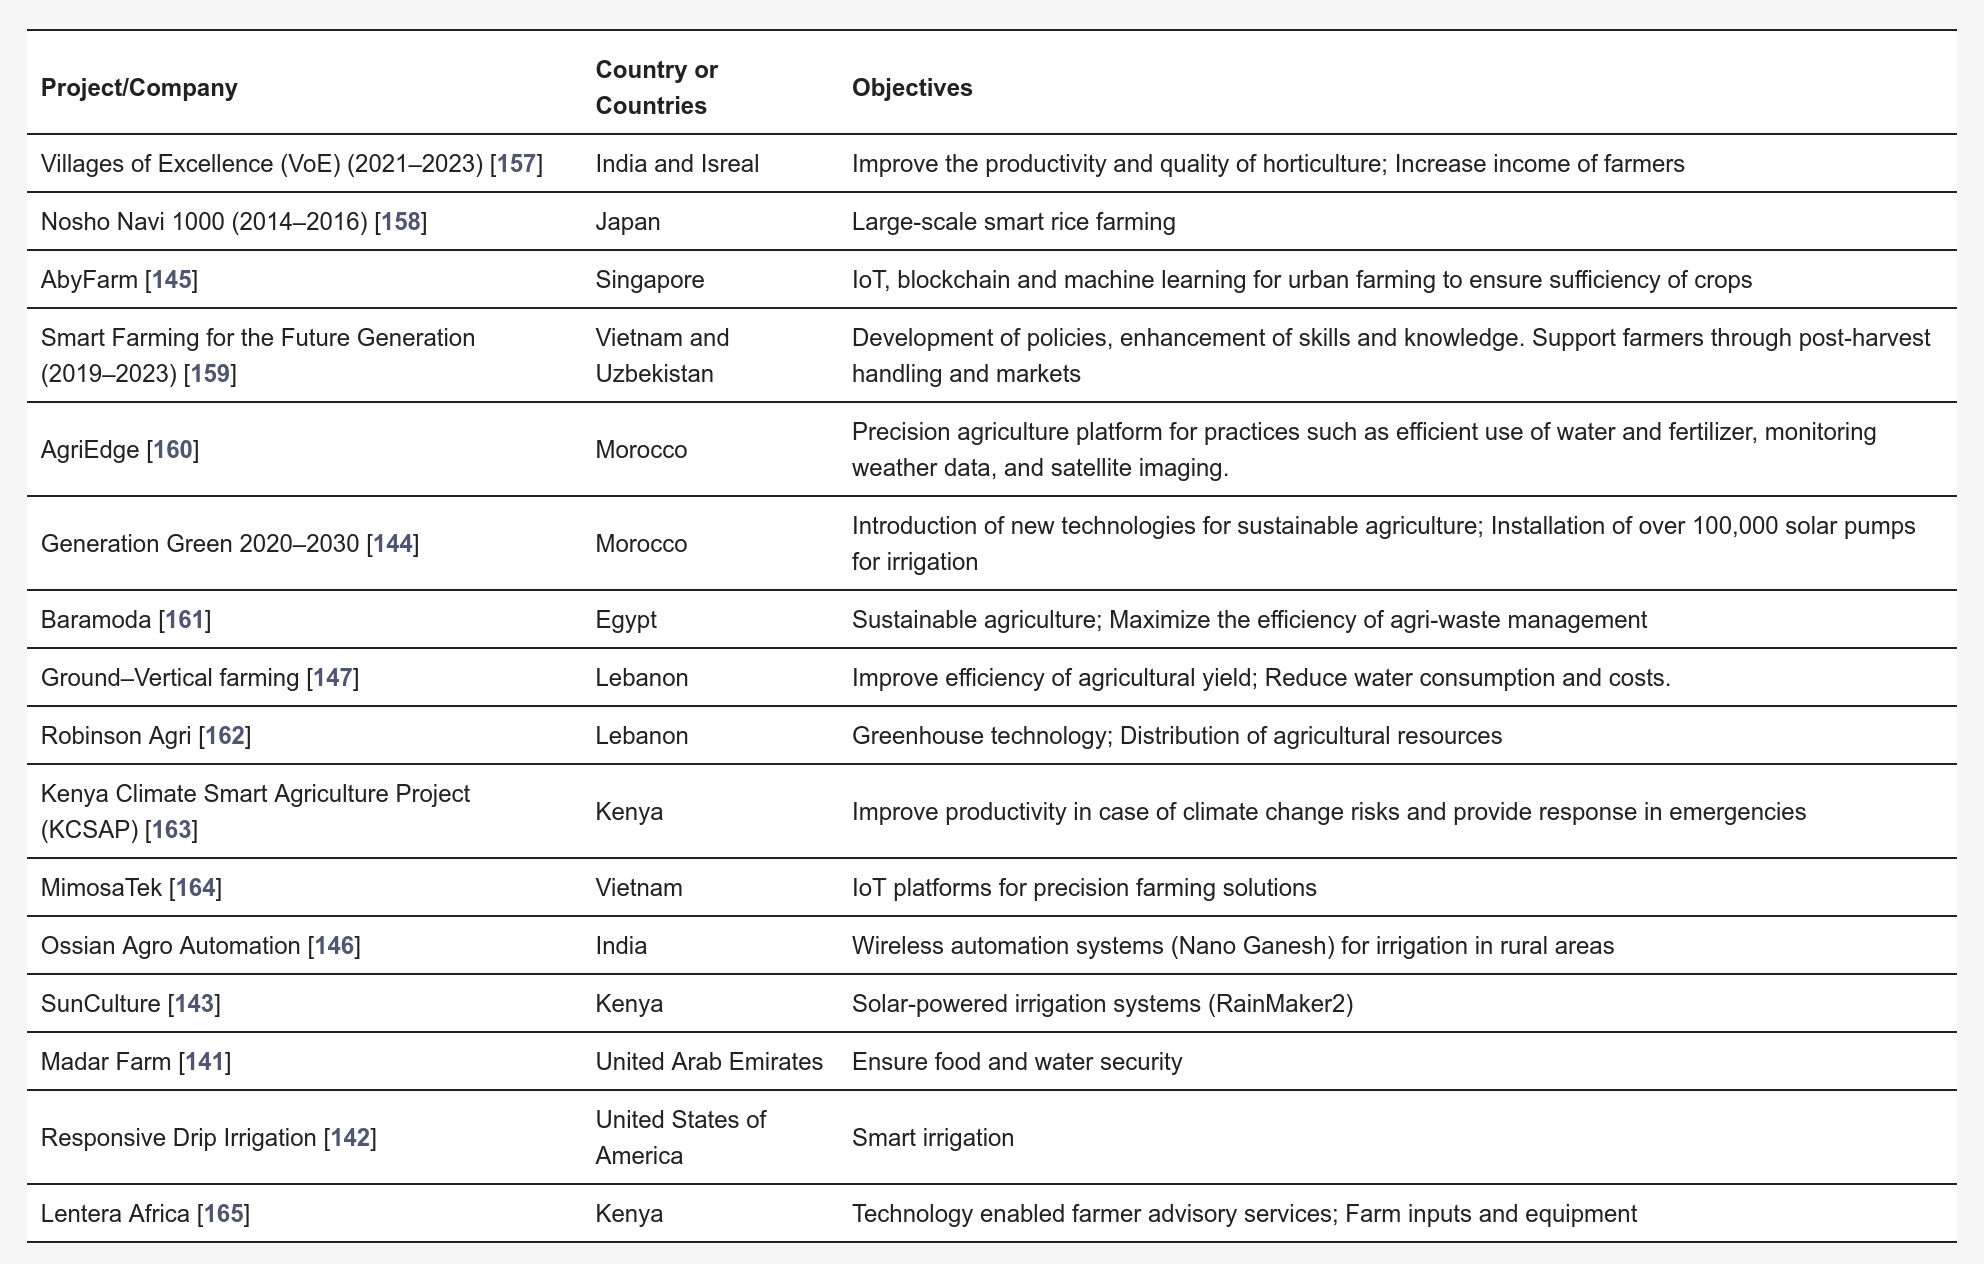
\includegraphics[width=\columnwidth]{research-table}
    \caption{A list of worldwide projects related to the area of Digital Agriculture (from \cite{agriengineering4020029})}
    \label{fig:table-worldwide}
\end{figure}




\section{Tebaka Project Description}\label{sec:tebaka}
% general project descript, partenrs, period, structure, goals

The present research project aims to define a “platform” solution for crops of grain, vines and olive oil, all of which are significantly present in the Puglia region, and will operate through stages of knowledge development and design / realization of prototype solutions that is articulated in the following basic structure:

Analysis of the territory of Puglia, identification of the areas and parcels cultivated to observe, definition / authorization of the operational missions and their verification.
Definition of payload and cargo platforms of sensors to be used (on already operational satellites and on aircraft and land systems to integrate / develop), development of a control room for mission management and operational integration with a data acquisition and processing center.
Definition of data acquisition criteria from various platforms / pay loads during the various missions envisaged, verification of operational adequacy in the identified territories and basic processing of acquired data through representation in thematic maps.
Definition of the theoretical models of the annual production cycles of the agricultural crops considered, of the fusion criteria of data from multisensor sources, of the criteria for the analysis of the data acquired in the missions, of the criteria for the realization of the data driven models with the use of artificial intelligence logic and deep learning, of criteria for their integration with theoretical models, and the implementation of integrated and validated basic models.
Development of Intensive Data Acquisition Activity from Payloads / Platforms for refinement of models, realized by means of large amounts of data processing, definition of criteria for identifying potential critical factors and development of models / support decision systems for their management, development of the design and the prototype of the complete system.
transversally to all projects of which DTA is the leader, consistent with the objectives of the Notice and the commitments that the proposers are required to sign with MIUR, will allow the evaluation and exploitation of the results, intermediate and final, valorization and dissemination within the communities of reference, the identification and application of methods and tools capable of maximizing the effects of public and private investment.
 
\lipsum[2-4]

\subsection{Results}

Realization of the prototype of an integrated platform composed of technological systems (satellites, manned and unmanned aircrafts, manned and unmanned land vehicles and fixed stations, payloads of sensors with different characteristics and performance, storage environments of large amounts of data and applications in the field of artificial intelligence for data manipulation, the building of data driven models, the development of models and relationships between the observed phenomena elements realized with machine learning logic, data analysis, decision support systems) in order to develop a product / service for the world of crops with different types of extension on the territory (horizontal for grain, vertical for vine and mixed for the olive tree, others with comparable characteristics) to be offered to various actors operating in the world of innovative agriculture such as Public Organizations, Category Associations, Service Providers, Agricultural Companies d medium / large national and international levels, possibly complementing the proposed solution with other complementary existing or developing ones.

The constitution of the advisory board presented is the basis for both orienting / validating the proposed solution and disseminating the product / service proposal to the agricultural world that is increasingly recognizing and utilizing intelligent agriculture solutions for the optimization of missions of the various actors involved.

During the development of the project, a comparison will be made between the participants and external stakeholders to evaluate the possibility / opportunity to realize a spin-off that, through the acquisition of the platform, can to industrialize, maintain and use it as a basis for providing advice / services on the market.

\lipsum[2-4]

\subsection{Goal}

The proposed project has as its ultimate goal the creation of an innovative product / service prototype for agriculture, in particular for grain, olive and vine crops, oriented to provide instruments and knowledge for the acquisition and to generate information for management decisions, in particular to provide guidance in the initial stages of potential and / or critical manifestations and to guide the best-performing actions.


It is primarily usefull for large territorial use but still maintains its validity for smaller areas, encouraging in this regard the concept of joint use among multiple actors in order to benefit from innovative solutions through affordable costs.


The concept of working with models of annual production cycles also allows to better estimate the final industrial result, and therefore economic, of the productions in progress.


The solution enables both private and public entities to design high value added services. For private sector it can be usefull for consultancy while for the public actors it can support policies and actions in order to favour the development of the agricultural production.


The articulation of activities, and hence the results that can be achieved for each one, also creates value in both the realization / improvement of system components (better bid ability in their business markets) and the development of internal knowledge and capabilities to be used also for development of other products / services / solutions.


The greatest knowledge gained from the university and research entities can also offer better and consulting skills in the market, also contributing to the enhancement of the territory.

\lipsum[2-3]

\section{Project Activities}\label{sec:activities}
% main part: flow of activities, from observation to 
% practical agronomic practice.

\subsection{Remote Sensing and Observation}
% remote sensing platforms, big players, open satellite data.
% impact and use of them, spectral indexes, IoT, smart
% deployment. Web app for agronomy, for field data collection.

\lipsum[2-10] %<- to be filled

\subsection{Machine Learning in Agritech}
% Image analysis using deep learning, role, goals result.

\lipsum[2-10]  %<- to be filled

\section{Related Works}\label{sec:related}
% a panoramic view of the best literature, focus on technology.

In \cite{LiSurvey2021,Adao2017} we have...

\lipsum[2-8] 

\section{Conclusion}\label{sec:conclusion}
\lipsum[1-3]

\section*{Acknowledgment}
 Put sponsor 
acknowledgments in the unnumbered footnote on the first page.

\printbibliography

\end{document}
